\documentclass[12pt]{article}
\usepackage[latin1]{inputenc}
\usepackage{amsmath}
\usepackage{amsfonts}
\usepackage{amssymb}
\usepackage{setspace}
\usepackage{enumitem}
\usepackage{verbatim}
\usepackage{amsthm}
\usepackage[table]{xcolor}% http://ctan.org/pkg/xcolor
\usepackage{graphicx}
\usepackage{color}
\usepackage{tabularx}  % for 'tabularx' environment and 'X' column type
\usepackage{algorithm,algorithmic}
\newtheorem{definition}{Definition}
\newtheorem{theorem}{Theorem}
\usepackage{filecontents}
\usepackage{lineno}
\usepackage{authblk}
%\linenumbers
\usepackage[margin=1.in]{geometry}
\usepackage[authoryear]{natbib}
\usepackage[hidelinks]{hyperref}

\title{
Geodetic First Approximation of Size and Timing: \\ User's Guide
}
\author[1]{Brendan Crowell \thanks{crowellb@pnsn.org}}
\author[2]{Ben Baker \thanks{benbaker@isti.com}}
\affil[1]{Pacific Northwest Seismic Network}
\affil[2]{Instrumental Software Technologies, Inc.}
\renewcommand\Authands{ and }
\date{\today}

\begin{document}
\maketitle
\tableofcontents

\clearpage
\section{Introduction}
copy brendan's original manual, note the amazon funding, and add brendan's publications
so people know what to cite  

G-FAST (Geodetic First Approximation of Size and Timing) was developed by Brendan Crowell
as a Python based geodetic earthquake early warning (EEW) module.  Funding from Amazon has
allowed PNSN to developed a compiled-language production variant of G-FAST for integration 
into the USGS's next generation ShakeAlert EEW system.  The software is released under the 
license described in Appendix \ref{s:license}.

Nominally, G-FAST acquires real-time geodetic data and, when triggered by a ShakeAlert
message, activates three geodetic co-seismic inversion suites: a peak ground displacement 
(PGD) inversion, a centroid moment tensor (CMT) inversion, and a CMT driven slip or finite fault
inversion.  The PGD module provides a quick and robust estimate of magnitude.  
The CMT inversion provides a robust estimate of magnitude, depth, and moment tensor
components.  The moment-tensor derived fault planes and depth are then passed onto the
slip inversion which resolves the CMT fault plane ambiguity while providing an 
additional magnitude estimate.  The PGD and slip model are then passed onto the
ShakeAlert decision module as the event unfolds.  

As in the Python implementation, G-FAST still acquires real-time data from the Pacific
Northwest Geodetic Array (PANGA) and, in the EEW context, is triggered on ShakeAlert
messages.  The key differences are now that an Earthworm server is responsible for the
import of PANGA data and the ShakeAlert communication is directly implemented via  
ActiveMQ.  Additionally, G-FAST has been separated into multiple C-libraries to encourage
reuse by groups outside of EEW.  



 

\clearpage
\section{Installation}
This section outlines the GFAST installation procedure.  This consists of two primary steps.
The first step is to install the dependencies.  The second step is to then build GFAST and
link to the dependencies.    

\subsection{Prerequisites}
This section lists the requisite, optional, and workaround libraries for building GFAST.   

\subsubsection{Compilers} 
The following libraries and GFAST can be compiled with a 
C, C++, and Fortran compiler.  It is recommended the compilers have complete 
\href{http://openmp.org/wp/}{OpenMP-4} support for improved code vectorization.  
OpenMP-4 support is realized in GCCv5 and above or Clang 3.9 and above though GFAST has
been successfully built with GCCv4.4.  If using GCCv4 then it is
recommend one set the ``-Wno-unknown-pragmas'' C compiler flag.

\subsubsection{CMake} CMake is used because G-FAST is decomposed into many smaller libraries with 
varying dependencies.  This dependency ambiguity is implicitly handled by this automatic 
makefile generator. In addition to generation of makefiles also CMake provides for automatic generation
and execution of unit tests. As with any makefile creation step the correct 
specification of dependencies can be quite painful but, upon successful generation of a
CMakeCache.txt, file this activity need not be repeated and subsequent pulls from the git
repository should build without hassle.  CMake is likely available through a package manager
or can be obtained from \url{https://cmake.org/}.  GFAST has been successfully built with
Version 2.6 and above.  

\subsubsection{LAPACK and BLAS} G-FAST ultimately aims to solve matrix-vector
equations of the form $\Vert G \textbf{m} = \textbf{d}\Vert_2 $ (LAPACK) or estimate 
data by computing matrix-vector multiplies of the form $\textbf{u} = G \textbf{m}$ (BLAS).  
Moreover, profiling shows that computation of the least-squares problem, particularly in the
finite fault inversion, is the greatest contributor to program execution time.  
Necessarily, one can easily achieve better performance
by using high-performance vendor LAPACK and BLAS library implementations.  
Consequently, it is recommended one follow the strategy of 
\begin{enumerate}
  \item Check for an existing vendor LAPACK/BLAS implementation.  
  \item If using an Intel processor obtain Intel's Math Kernel Library (MKL) 
        which is freely available at \url{https://software.intel.com/sites/campaigns/nest/}.
        Also, note that MKL contains an implementation of FFTw and may reduce the number of
        dependencies. 
  \item Check a package manager for a pre-built LAPACK and BLAS which are distributed with a
  modified BSD license.
  \item TODO: look for OpenBLAS then, if not found, ATLAS in the CMakeModules if using a 
  package manager's lapacke + blas.      
  \item At last resort obtain and build LAPACK and BLAS from \url{http://www.netlib.org/lapack/}
  which are distributed with a modified BSD license. 
\end{enumerate}

\subsubsection{libGeographic}
This is a library used by GFAST's coordinate tools unit tests.  It may be available through
a package manager or, if need be, obtained from \url{http://geographiclib.sourceforge.net/}.  It is
distributed under the MIT license. 

\subsubsection{iniparser}
This is the utility which parses the GFAST parameter file.  It is available from
\url{https://github.com/ndevilla/iniparser} and is distributed under the MIT license.

\subsubsection{HDF5}
The HDF5 self-describing file format is used for high-performance and portable data archival and
data playback.  HDF5 can be obtained from a package manager or from 
\url{https://www.hdfgroup.org/HDF5/}. 
GFAST appears to work with HDF5 1.18.6.  If static linking to HDF5 then one must additionally 
obtain the zlib compression library.  A zlib implementation is available in Intel's 
Performance Primitives available at \url{https://software.intel.com/sites/campaigns/nest/}.  Zlib
can also be obtained with a package manager or from \url{http://www.zlib.net}.  
Notice that there is no data compression in GFAST disk writes and this step can be avoided by
linking to the shared HDF5 library.  If choosing between IPP and a zlib then note that
IPP improves the performance of ISCL.   Zlib and HDF5 both are distributed with permissive
software licenses.

\subsubsection{libxml2}
The ShakeAlert and QuakeML data products are created with libxml2.  If using GCC then it
is very likely you already have libxml2.  Otherwise, it can be obtained from 
\url{http://xmlsoft.org/}.  libxml2 is distributed under the MIT license. 

\subsubsection{ISCL}
Brendan's initial GFAST implementation was written in Python and made extensive use of 
Numerical Python.  Somewhat fortuitously ISTI had been developing a library targeted 
at expediting the conversion of NumPy laden Python scripts to C via the ISTI Scientific
Computing Library (ISCL).  ISCL is distributed under the Apache-2 license and 
freely available from \url{https://github.com/bakerb845/libiscl}.

\subsubsection{ActiveMQ}
The ShakeAlert earthquake early warning system sends and receives alerts with the ActiveMQ
messaging system.  If one is not using GFAST in earthquake early warning then ActiveMQ
is not necessary.  ActiveMQ additionally depends on libcrypto and libssl.  ActiveMQ is
distributed under the Apache 2 license is available at
\url{http://activemq.apache.org/cms/download.html}. 

\subsubsection{Earthworm}
The real-time GPS data are currently incorporated into GFAST via Earthworm which is
available at \url{http://earthworm.isti.com/trac/earthworm/}.  If not using the real-time
system then Earthworm is not necessary.  Earthworm requires two
additional libraries, RabbitMQ-c and Jansson for import of the GeoJSON which contains the GPS
precise-point-position data.  RabbitMQ-c 
is available at \url{https://github.com/alanxz/rabbitmq-c} and is distributed with an 
MIT license.  Jansson is available at \url{https://github.com/akheron/jansson} and
is distributed with a permissive license. 

\subsubsection{FFTw}
The requirement for this library will be dictated by your linking policy.  If you require 
static linking \emph{and} are not using Intel MKL then to successfully build GFAST you would 
have to obtain FFTw from a package manager or obtain it from \url{http://www.fftw.org/}.
Notice however that no Fourier transforms are computed in GFAST.  Additionally, if static
linking without MKL then FFTw's GPL-2 copyleft will impact GFAST's internal license.
To avoid this complication it is recommended one use MKL or link to the dynamic ISCL library.  

\subsubsection{Cython}
A developmental Python interface is provided through Cython which converts Python to C and is 
available at \url{http://cython.org/} or through a package manager.  This is not required and
at the present time minimally supported.

\subsubsection{cMoPaD}
The moment tensor decompositions are accomplished through a C implementation of 
\href{https://github.com/geophysics/MoPaD}{MoPaD}.  This is distributed with GFAST.  
Because the C implementation is derivative work it must assume MoPaD's original 
LPGL3 license.  This means that one can safely link to the shared MoPaD library without
modifying the GFAST license.  This is reflected in the target link library of the 
src/CMakeLists.txt  file.

\subsection{Building G-FAST}

To increase the likelihood that G-FAST can be compiled on multiple platforms (e.g. Linux, 
Windows, OSX) and ease the burden on developers to modify cumbersome makefiles G-FAST 
adopts the \href{https://cmake.org/}{CMake} automatic makefile generation utility.  
Naively, one can descend into G-FAST's root directory and type 
\begin{verbatim}
cmake .
\end{verbatim}  
The CMakeModules will attempt to find the requisite libraries and may be moderately successful
if items are installed in `standard' locations.  

Alternatively, if one would prefers a less serendipitous build then the paths to the custom
directories can be provided directly to cmake  
\begin{verbatim}
cmake ./ -DCMAKE_BUILD_TYPE=DEBUG \
      -DCMAKE_INSTALL_PREFIX=./ \
      -DCMAKE_C_FLAGS="-g3 -O2 -fopenmp -Wall -Wno-unknown-pragmas" \
      -DEW_BUILD_FLAGS="-Dlinux -D_LINUX -D_INTEL -D_USE_SCHED  -D_USE_PTHREADS" \
      -DCMAKE_CXX_FLAGS="-g3 -O2" \
      -DUSE_AMQ=TRUE \
      -DGFAST_USE_EW=TRUE \      
      -DAPR_INCLUDE_DIR=path_to_include_apr-1 \
      -DLIBAMQ_INCLUDE_DIR=path_to_include_activemq-cpp-3.8.2 \
      -DLIBAMQ_LIBRARY=path_to_libactivemq-cpp \
      -DLSSL_LIBRARY=path_to_libssl \
      -DLCRYPTO_LIBRARY=path_to_libcrypto \
      -DLAPACKE_INCLUDE_DIR=path_to_lapacke_include \
      -DLAPACKE_LIBRARY=path_to_liblapacke \
      -DLAPACK_LIBRARY=path_to_liblapack \
      -DCBLAS_INCLUDE_DIR=path_to_cblas_include \
      -DCBLAS_LIBRARY=path_to_libcblas \
      -DBLAS_LIBRARY=path_to_libblas \
      -DH5_C_INCLUDE_DIR=path_to_hdf5_include \
      -DH5_LIBRARY=path_to_libhdf5 \
      -DINIPARSER_INCLUDE_DIR=path_to_iniparser_src \
      -DINIPARSER_LIBRARY=path_to_libiniparser \
      -DISCL_INCLUDE_DIR=path_to_iscl_include \
      -DISCL_LIBRARY=path_to_libiscl_static \
      -DGEOLIB_LIBRARY=path_to_libGeographic \
      -DFFTW3_LIBRARY=path_to_libfftw3 \
      -DEW_INCLUDE_DIR=path_to_earthworm_include \
      -DEW_LIBRARY=path_to_earthworm_libew \
      -DLIBXML2_INCLUDE_DIR=path_to_libxml2 \
      -DLIBXML2_LIBRARY=path_to_libxml2
\end{verbatim}
As another example, one can use the MKL and IPP libraries to boost performance 
\begin{verbatim}
cmake ./ -DCMAKE_BUILD_TYPE=DEBUG \
      -DCMAKE_INSTALL_PREFIX=./ \
      -DCMAKE_C_COMPILER=/usr/bin/gcc-5 \
      -DCMAKE_CXX_COMPILER=/usr/bin/c++ \
      -DCMAKE_C_FLAGS="-g3 -O2 -fopenmp -Wall" \
      -DEW_BUILD_FLAGS="-Dlinux -D_LINUX -D_INTEL -D_USE_SCHED  -D_USE_PTHREADS" \
      -DCMAKE_CXX_FLAGS="-g3 -O2" \
      -DGFAST_USE_INTEL=TRUE \
      -DUSE_AMQ=TRUE \
      -DGFAST_USE_EW=TRUE \      
      -DAPR_INCLUDE_DIR=path_to_apr \
      -DLIBAMQ_LIBRARY=path_to_libactivemq-cpp \
      -DLSSL_LIBRARY=path_to_libssl \
      -DLCRYPTO_LIBRARY=path_to_libcrypto \
      -DMKL_LIBRARY="mkl;libraries;" \
      -DIPP_LIBRARY="intel;performance;libraries" \
      -DH5_C_INCLUDE_DIR=path_to_hdf5_include \
      -DH5_LIBRARY=path_to_lib_libhdf5 \
      -DINIPARSER_INCLUDE_DIR=path_to_iniparser_src \
      -DINIPARSER_LIBRARY=path_to_libiniparser \
      -DISCL_INCLUDE_DIR=path_to_iscl_include \
      -DISCL_LIBRARY=path_to_libiscl \
      -DGEOLIB_LIBRARY=path_to_libGeographic \
      -DEW_INCLUDE_DIR=path_to_ewinclude \
      -DEW_LIBRARY=path_to_libew \
      -DLIBXML2_INCLUDE_DIR=path_to_libxml2_include \
      -DLIBXML2_LIBRARY=path_to_libxml2
\end{verbatim}
In both instances the Earthworm pre-processor flags were obtained from the appropriate
${GLOBALVARS}$ as to be consistent with Earthworm headers. 

Note, the above examples provide the option of building with ActiveMQ and Earthworm.  This
behavior is controlled through the DUSE\_AMQ and DUSE\_EW flags respectively.  If either flag
is not set then the default behavior should be to false.  This may be advantageous when
building GFAST in a pure playback mode of operation.  In this case one would not need to 
specify the corresponding ActiveMQ and Earthworm library and include directories.  

\subsection{Generating the Doxygen Documentation}
\href{http://www.stack.nl/~dimitri/doxygen/}{Doxygen}
is a useful tool for generating a type of code documentation.  It is particularly
useful to developers who wish to look-up variables in structures, variable meanings in 
function calls, and program function dependencies.  Doxygen is unobtrusively used by
decoarting preambles in source files and structures in header files.  After running
doxygen on the Doxyfile in the root source directory, Doxygen will scan the predetermined
source folders and autogenerate a large amount of documentation.  The output can be viewed
with a web-browser or PDF viewer.  

\clearpage
\section{G-FAST Library Overview}
This section will outline the G-FAST libraries as summarized in Figure \ref{F:gfastOverview}.  
Libraries are used extensively 
to emphasize modularity, allow users to customize G-FAST to their application 
without incurring the cruft of another G-FAST application, and promote a maintainable
software framework whereby software fixes can efficiently propagate to all users.  
The libraries to be introduced are
\begin{itemize} 
 \item Subsection \ref{ss:gfastCore}: libgfast\_core for core G-FAST modeling and inversion  
 \item Subsection \ref{ss:gfastActiveMQ}: libgfast\_activeMQ for G-FAST communication in ShakeAlert
 \item Subsection \ref{ss:gfastHDF5}: libgfast\_hdf5 for G-FAST archival of heavy data
 \item Subsection \ref{ss:gfastXML}: libgfast\_xml for parsing and generating QuakeML and ShakeAlert XML
 \item Subsection \ref{ss:gfastTraceBuffer}: libgfast\_traceBuffer for data IO from Earthworm and HDF5
 \item Subsection \ref{ss:gfastMopad}: libcmopad for moment tensor decompositions 
\end{itemize}

\begin{center}
\begin{figure}
\includegraphics[scale=0.45]{Figs/gfast_eew_overview.jpg}
\caption{Overview of G-FAST and its libraries.}
\end{figure}\label{F:gfastOverview}
\end{center}

\clearpage
\subsection{G-FAST Core Routines}\label{ss:gfastCore}
This section outlines the libgfast\_core utilities which are essential to the expert
earthquake-early warning driver routines.  The six primary utilities are
\begin{itemize}
  \item A properties reader for requisite G-FAST modeling parameters.
  \item Waveform processing for computation of peak ground displacement or offsets
  derived from precise-point-position time series data.
  \item PGD inversion of peak ground displacement data computed in the waveform processing.
  \item CMT inversion of offset data computed in the waveform processing.
  \item Finite fault inversion of data computed in the waveform processing.
  \item Coordinate utilities for converting latitude and longitude to and from 
  UTMs\footnote{This directory supersedes the libGeographic ISCL interface as libGeographic 
            has unpredictable behavior when crossing UTM zones that could jeopardize
            program library execution in the Pacific Northwest.}.   
  \item An event list handler for handling multiple events.
\end{itemize}

\subsubsection{G-FAST Properties Reader}
The G-FAST properties directory is responsible for reading all properties from the 
G-FAST properties file.  To mimic the functionality of G-FAST will have general
properties, PGD scaling properties, CMT inversion properties, finite-fault inversion properties.
and, optionally, ActiveMQ properties and Earthworm properties.  
The properties will be discussed at greater length in
Section \label{S:propertiesFile}.  In this directory also exists a convenience routine for
clearing the G-FAST properties during a finalization phase as well as displaying the properties
to a text file or standard out.

\subsubsection{G-FAST PGD Scaling}
The G-FAST peak ground displacement inversion accepts from the waveform processor the
largest\footnote{Largest is maximum observed Euclidean distance of the three-component offset 
data within a valid S-wave mask.} peak ground displacements in a valid region around the
earthquake hypocenter.  This valid region is computed from a configurable S-wave masking velocity to
prevent offsets at different stations from contaminating the inversion.  From this PGD data, 
G-FAST will 
\begin{equation}
 gm=u
\end{equation}

\subsubsection{G-FAST CMT Inversion}
The G-FAST CMT inversion accepts from the waveform processor average static offsets for each station
and component from the time a theoretical S-wave has passed through the station to the latest available
data point.  Like in the PGD scaling the CMT S-wave mask velocity is configurable.  Provided the
theoretical S-wave has passed through a configurable minimum number of stations the inversion will
perform for each depth a linearized moment tensor inversion.  The moment tensor inversion is 
constrained to purely deviatoric sources for stability.  
\begin{equation}
  G \hat{\textbf{m}} = \textbf{d}
\end{equation}
where 
\begin{equation}
   \hat{\textbf{m}} 
 = \left \{ 
     \begin{array}{c} 
       m_{xy} \\ m_{xz} \\ m_{zz} \\ \frac{m_{xx} - m_{yy}}{2} \\ m_{yz} 
     \end{array}
   \right \}
\end{equation}
and 
\begin{equation}
  G =
\end{equation}
As a word of caution, observe that the output moment tensors have been converted to a
more conventional North, East, Down \citep[e.g.][]{jostAndHerrmann} 
$\{m_{xx}, m_{yy}, m_{zz}, m_{xy}, m_{xz}, m_{yz}\}^T$ for the HDF5 output 
and Up, South, East
\citep[e.g.][]{globalCMT} 
$\{m_{rr}, m_{\theta \theta}, m_{\phi \phi}, m_{r \theta}, m_{r \phi}, m_{\theta \phi} \}^T$
for the QuakeML output.  

After the grid-search is complete a double-couple promoting penalty is applied at each depth,
$i=1,2,\cdots, n_{d}$, to the variance reduction, $v_r^{(i)}$ 
\begin{equation}
  \hat{v_r}^{(i)} = \frac{v_r^{(i)}}{\operatorname{DCP}\{\textbf{m}^{(i)}\}}
\end{equation}
where $\operatorname{DCP}$ denotes the double couple percentage of the moment tensor.  

\subsubsection{G-FAST Finite Fault Inversion}

\subsubsection{G-FAST Event Handler}
In real-time applications it is possible multiple events can occur within a modeling window.  
To accomodate this G-FAST has a small facility for event bookkeeping that
relies on the assumption that all events have unique event IDs.  
These functions can add a new event to the processing list or remove an event if it has surpassed
its maximum modeling time (expired), or remove an event if its event ID was cancelled.

\subsection{G-FAST ActiveMQ Messaging}\label{ss:gfastActiveMQ}
The ShakeAlert framework requires a flexible message service to allow different modules to
communicate.  This is realized with the ActiveMQ library.  G-FAST makes very limited use of
ActiveMQ for EEW ShakeAlert compliance.  G-FAST can subscribe to a message queue whereby it
consumes XML messages from the decision module.  
G-FAST can also subscribe to a message queue to which it produces XML messages for future 
ShakeAlert use.  To use both features one mess correctly enter the credentials specified
in the properties file. 

\subsection{G-FAST HDF5 Archive}\label{ss:gfastHDF5}
Presently there exists a framework for creation and dissemination of ShakeAlert products via
XML.  However, as an algorithm's products and complexity increasses it becomes important to consider
frameworks for saving the heavy data in the applications highspeed memory to disk.  This is
accomplished in a portable and flexible way with self-describing binary HDF5 file format.  Using
HDF5 can copy then write to disk each application data structure for every G-FAST iteration.

\subsection{G-FAST XML Creation and Parsing}\label{ss:gfastXML}
The eXtensible Markup Language format is a portable human and machine readable file format
used by ShakeAlert for communication of core data products (e.g., hypocenter, origin time, magnitude).  
G-FAST and the other geodetic algorithms will extend the core products to include magnitudes from
PGD inversion and fault slip inversions.  Additionally, because G-FAST computes CMTs, G-FAST
will offer an XML based earthQuake Markup Language (quakeML) CMT summary which may be of use to
NEIC earthquake contributors.  

\subsection{G-FAST Trace Buffers}\label{ss:gfastTraceBuffer}
G-FAST is intended for use in both real-time and purely playback scenarios with the underlying
assumption that it was not to be an Earthworm module.  To achieve this flexibility a common HDF5 
data file format serves as an application middleware.  This library is responsible for accessing
the common H5 file format.  Additionally, when using G-FAST in a real-time scenario, this library
has the necessary functionality for reading the Earthworm rings and and updating the HDF5 data file.
Note, the CMake has been designed so that the Earthworm can quickly be ejected if it one only 
desires to use G-FAST in a playback mode or implement another datasource such as SeedLink.   
This library is summarized at a high level in a real-time application by Figure \ref{F:gfastDataIO}.  

\subsection{Moment Tensor Decompositions with cMoPaD}\label{ss:gfastMopad}
At the time of writing G-FAST is the only proposed ShakeAlert module which can perform
moment tensor inversions.  A common feature in CMT inversions is the ability to decompose
the inverted moment tensor into isotropic, compensated linear vector dipole, and double
couple parts \citep[e.g.][]{jostAndHerrmann1989}.  Towards this end a flexible Python 
package was introduced by \citet{krieger} in \href{https://github.com/geophysics/MoPaD}{MoPaD}.  
ISTI has reimplemented the very general decomposition component of MoPaD in C for 
computational efficiency.  The primary utility of such a decomposition library in G-FAST is 
in the CMT gridsearch double-couple percentage weighting.  This library is also used in 
generation of a more complete QuakeML which describes a moment tensor in terms of fault planes 
as well as it's eigenvectors. 

One should observe ISTI's cMoPaD is by definition derivative work.  Consequently, this library
must be distributed under the L-GPL license.  The consequence is that any software statically
linking to this library must have a license which is L-GPL compatible.

\clearpage
\subsection{Data Acquisition}
This section outlines the data acquisition strategy in real-time and playback operations.
To make the real-time acquisition and playback appear integrated to the user a common
HDF5 file format is selected.  For playbacks, a pre-processing program can be used to generate 
a valid input data 
file\footnote{`File' is a generic word in the context of this discussion.  
It is unnecessary and potentially undesirable from a performance standpoint that
the file physically exist in the computer's disk space.  The illusion of keeping 
the file on disk is accomplished by instructing HDF5 to memory map the data 
file during the start-up phase.}
which is queried by a simple API for data in a given a time range.  
Likewise, real-time data is  
written\footnote{The writes can be to memory or disk.}
to an HDF5 file with the same structure as a playback data file and, like in playback mode,
can be queried by the same API as the playback for data in a given time range.

\begin{center}
\begin{figure}
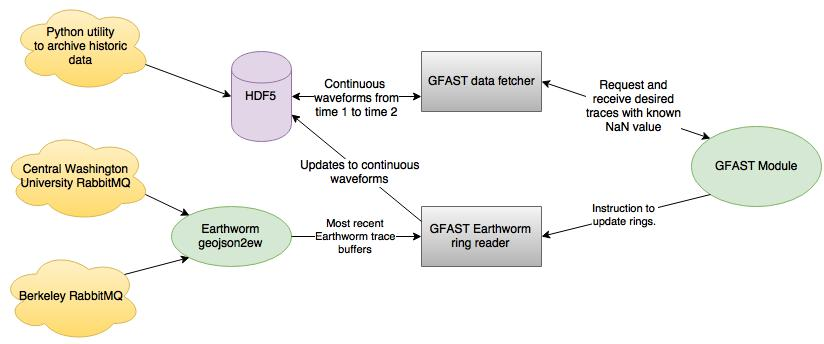
\includegraphics[scale=0.55]{Figs/gfast_dataIO.jpg}
\caption{A depiction of the current data flow.  The goal is to put the data in a common, 
continuous, finite-sized format hereby encapsulated by the HDF5 archive.  
In the context of playbacks the bottom functions are not used.
Hence, it is the same function that queries the HDF5 archive in playback and 
real-time mode and the G-FAST application developer is only exposed to one data 
fetcher API.  The API is very simple in that G-FAST specifies two times, for example 
the event origin time and the current time, and the data is returned with the understanding
some data may be latent or non-existent and have a predetermined value indicating its absence. 
For real-time scenarios the Earthworm acquisition must be configured 
and running prior to launching a G-FAST application.   The GPS data ring will be accessed
directly by a G-FAST function that relies on libew.a.  Real-time applications 
must additionally call the G-FAST ring reader function periodically, say every second, 
to refresh the HDF5 archive.
}\label{F:gfastDataIO}
\end{figure}
\end{center}



\clearpage
\subsection{XML Output}
This section outlines the three XML data products.  Two XML products, PGD and finite fault, have
defined ShakeAlert schemas.  The third XML product is a QuakeML summary CMT summary for potentially
expediting communication between the tsunami warning centers and NEIC. 

\clearpage
\subsection{HDF5 Output}
This section outlines the HDF5 summary files.  HDF5 is a portable and high performance 
utility which makes it possible to easily archive the results\footnote{Since results are 
encapsulated in data structures the HDF5 files are the data structures after each iteration.}
of G-FAST after each iteration thereby providing a snapshot of the GFAST execution and 

\section{Using G-FAST}
This section describes the G-FAST usage in layback application and earthquake early warning.  
There are three steps in a G-FAST.  The first step is creation of a parameter file and 
additional data files.  The second step is running the application.  The third step is
post-processing the resulting HDF5 summary file.

\subsection{The G-FAST Base Properties File}\label{S:propertiesFile}
This section describes the G-FAST parameters common to both playback and earthquake early warning.

The most recent metadata file can be obtained at 
\url{http://www.panga.cwu.edu/eew/readi_sites_metadata.txt}.  

\subsection{The G-FAST Playback Properties File}

\subsection{The G-FAST Earthquake Early Warning Properties File}

\section{Acknowledgements}
This software was developed with funds from the amazon catylyst and government grants a, b, c and d.  

\appendix
\section{License}\label{s:license}
brendan, you have to email the comotion (tech transfer) and see what they want.  
i'm going to guess this software belongs to uw, ideally it is free (as in beer) 
for academics and government organizations, you can freely modify the code however uw owns 
all modifications to the software, you cannot redistribute the code, the software
is provided as is, and you cannot hold uw liable.  i don't think gpl will be a good license
choice.  if this library is to exist in the shakealert framework gpl licensing can very easily 
find itself conflicting with caltech licensed software.  but that's the usgs's problem and not yours.   

\end{document}

